%%%%%%%%%%%%%%%%%%%%%%%%%%%%%%%%%%%%%%%%%%%%%%%%%%%%%%%%%%%%%%%%%%%%%%
% LaTeX Example: Project Report
%
% Source: http://www.howtotex.com
%
% Feel free to distribute this example, but please keep the referral
% to howtotex.com
% Date: March 2011 
% 
%%%%%%%%%%%%%%%%%%%%%%%%%%%%%%%%%%%%%%%%%%%%%%%%%%%%%%%%%%%%%%%%%%%%%%
% How to use writeLaTeX: 
%
% You edit the source code here on the left, and the preview on the
% right shows you the result within a few seconds.
%
% Bookmark this page and share the URL with your co-authors. They can
% edit at the same time!
%
% You can upload figures, bibliographies, custom classes and
% styles using the files menu.
%
% If you're new to LaTeX, the wikibook is a great place to start:
% http://en.wikibooks.org/wiki/LaTeX
%
%%%%%%%%%%%%%%%%%%%%%%%%%%%%%%%%%%%%%%%%%%%%%%%%%%%%%%%%%%%%%%%%%%%%%%
% Edit the title below to update the display in My Documents
%\title{Project Report}
%
%%% Preamble
\documentclass[paper=letter, fontsize=10pt]{scrartcl}
\usepackage[body={7in,7.5in},top=1in, bottom=1in]{geometry}
\usepackage[T1]{fontenc}
\usepackage{fourier}

\usepackage[english]{babel}															% English language/hyphenation
\usepackage[protrusion=true,expansion=true]{microtype}	
\usepackage{amsmath,amsfonts,amsthm} % Math packages
\usepackage[pdftex]{graphicx}	
\usepackage{url}
\usepackage{enumerate}
\usepackage{lastpage}
\usepackage{float}
\usepackage{hyperref}


%%% Custom sectioning
\usepackage{sectsty}
\allsectionsfont{\normalfont\scshape}


%%% Custom headers/footers (fancyhdr package)
\usepackage{fancyhdr}
\pagestyle{fancy}
\fancyhead[L]{}
\fancyhead[c]{Design Revision 0 Revision 0}
\fancyhead[R]{\today}											
\fancyfoot[L]{}											 
\fancyfoot[C]{}											
\fancyfoot[R]{\thepage\ of \pageref{LastPage}}		% Pagenumbering
\renewcommand{\headrulewidth}{0.4pt}				% Remove header underlines
\renewcommand{\footrulewidth}{0.4pt}				% Remove footer underlines
\setlength{\headheight}{13.6pt}


%%% Equation and float numbering
\numberwithin{equation}{section}		% Equationnumbering: section.eq#
\numberwithin{figure}{section}			% Figurenumbering: section.fig#
\numberwithin{table}{section}				% Tablenumbering: section.tab#


%%% Maketitle metadata
\newcommand{\horrule}[1]{\rule{\linewidth}{#1}} 	% Horizontal rule
\newcommand{\ts}{\textsuperscript}

%%% Begin document
\begin{document}

\begin{titlepage}

\newcommand{\HRule}{\rule{\linewidth}{0.5mm}} % Defines a new command for the horizontal lines, change thickness here
\newcommand{\authors}{\shortstack{Vitaliy Kondratiev,\\Nathan Johrendt,\\Tyler Lyn,\\Mark Gammie}}

\begin{center}
 
%----------------------------------------------------------------------------------------
%	HEADING SECTIONS
%----------------------------------------------------------------------------------------

\textsc{\LARGE McMaster University}\\[1.5cm] % Name of your university/college
\textsc{\Large CAS 4ZP6}\\[0.5cm]
\textsc{\Large Team 9} \\[0.5cm]
\textsc{\Large Capstone Project 2013/2014}\\[0.5cm] % Major heading such as course name
\textsc{\large Porter Simulation}\\[0.5cm] % Minor heading such as course title

%----------------------------------------------------------------------------------------
%	TITLE SECTION
%----------------------------------------------------------------------------------------

\HRule \\[0.4cm]
{ \huge \bfseries Design Revision 0}\\[0.4cm] % Title of your document
\HRule \\[1.5cm]
 
%----------------------------------------------------------------------------------------
%	AUTHOR SECTION
%----------------------------------------------------------------------------------------

\begin{minipage}{0.4\textwidth}
\begin{flushleft} \large
\emph{Authors:}\\
Vitaliy Kondratiev - 0945220\\
Nathan Johrendt - 0950519\\
Tyler Lyn - 0948978\\
Mark Gammie - 0964156\\
\end{flushleft}
\end{minipage}
~
\begin{minipage}{0.4\textwidth}
\begin{flushright} \large
\emph{Supervisor:} \\
Dr. Douglas Down % Supervisor's Name
\end{flushright}
\end{minipage}\\[4cm]

% If you don't want a supervisor, uncomment the two lines below and remove the section above
%\Large \emph{Author:}\\
%John \textsc{Smith}\\[3cm] % Your name

%----------------------------------------------------------------------------------------
%	DATE SECTION
%----------------------------------------------------------------------------------------

{\large \today}\\[3cm] % Date, change the \today to a set date if you want to be precise

%----------------------------------------------------------------------------------------
%	LOGO SECTION
%----------------------------------------------------------------------------------------

%\includegraphics{Logo}\\[1cm] % Include a department/university logo - this will require the graphicx package
 
%----------------------------------------------------------------------------------------
%Template taken from: http://www.softwaretestinghelp.com/test-plan-sample-softwaretesting-and-quality-assurance-templates/

\vfill % Fill the rest of the page with whitespace
\end{center}
\end{titlepage}

\setcounter{tocdepth}{2}

\tableofcontents

\newpage

\section{Revision History}
\begin{center}
    \begin{tabular}{| c | l | l | p{5cm} |}
    \hline
    Revision \# & Author & Date & Comment \\ \hline
  	1 & \shortstack{\\Vitaliy Kondratiev,\\Nathan Johrendt,\\Tyler Lyn,\\Mark Gammie} & January 11, 2014 & Revision 0 Added to repository \\ \hline
  	2 & \shortstack{\\Vitaliy Kondratiev,\\Mark Gammie} & January 12, 2014 & Added diagrams to Latex \\ \hline
  	3 & \shortstack{\\Tyler Lyn} & January 12, 2014 & Added dispatch module \\ \hline
  	4 & \shortstack{\\Vitaliy Kondratiev,\\Nathan Johrendt} & January 13, 2014 & Added GUI Component to document \\ \hline
  	5 & \shortstack{\\Mark Gammie} & January 13, 2014 & Updated Dependency Diagram to contain algorithms and data structures. Updated dependency diagram with a legend, logging comment and fixed the porter dispatcher dependency \\ \hline
  	6 & \shortstack{\\Tyler Lyn,\\Mark Gammie} & January 13, 2014 & Several Modules Updated \\ \hline
	7 & \shortstack{\\Nathan Johrendt} & January 13, 2014 & Added Appendix \\ \hline
	8 & \shortstack{\\Mark Gammie} & January 14, 2014 & Completed Design Overview\\ \hline
        
    \end{tabular}
\end{center}

\section{Executive Summary}
\subsection{Introduction}
This document outlines the design decisions, style and methodology for the project of Porter Simulation to be completed for Hamilton Health Sciences.  A modular design methodology has been chosen as our design principle.  This document is based on IEEE Draft Standard for Software Design Descriptions (IEEE P1016/D5.0).
\subsection{Purpose}
The purpose of this document is to outline the design of each component and how they interface between each other. This document will aid the developers in the development process as well as any future maintenance required.
\subsection{Design Overview}
Our solution is a discrete event simulation that is implemented using the Python library SimPy. The simulation has three main sections named Import, Export and Core. 

The Import section contains modules for accessing two different csv files that are used as input for the simulation. The first file contains a collection of data that has been exported from Hamilton Health Science's porter management system. The second file contains data that represents the work schedule of each porter that will be used in the simulation. Both of these files will be modified using Excel as the interface.

The Export section contains a module for reporting statistics that are generated by the simulation. The module will be used after the simulation has completed to write the generated data to a csv file that will be interpreted later by some Visual Basic scripts. These scripts will be used to generate predetermined graphs for the user to view.

The Core section is where the simulation actually occurs. The module Simulation Core contains the command line interface for the simulation and is responsible for initializing the Simulation State, Job List Builder and Dispatcher modules. The Job List Builder module will create a list of jobs using the data contained in the file filled with historical data. This list of jobs will be submitted to the Simulation State to be stored. Once the simulation is started, the Dispatcher module is responsible for receiving the jobs as they become available and assigning them intelligently to any eligible porters. The porters that operate on the tasks follow a finite state machine that creates timeouts based on the time it would take for each state that the porter is transitioning into. There may be cases when all the porters are busy and the amount of assigned jobs piles up, or the porters are stuck waiting on jobs to become available. Once the simulation terminates, the export of the statistical data is finalized.
\section{Implementation Material}
\subsection{Language of Implementation}
Visual Basic in Excel will be used to interface GUI to Simulation Core module. Python Version 2.7.5 will be used for Simulation Core module and all other modules.
\subsection{Supporting Technology and Frameworks}
Simulation will be built on the SimPy 3.0.2 library \newline \ \underline{\url{https://simpy.readthedocs.org/en/latest/}}. GUI will be built in Excel 2010. 

\section{Process Diagram}
\begin{figure}[H]
	\begin{center}
		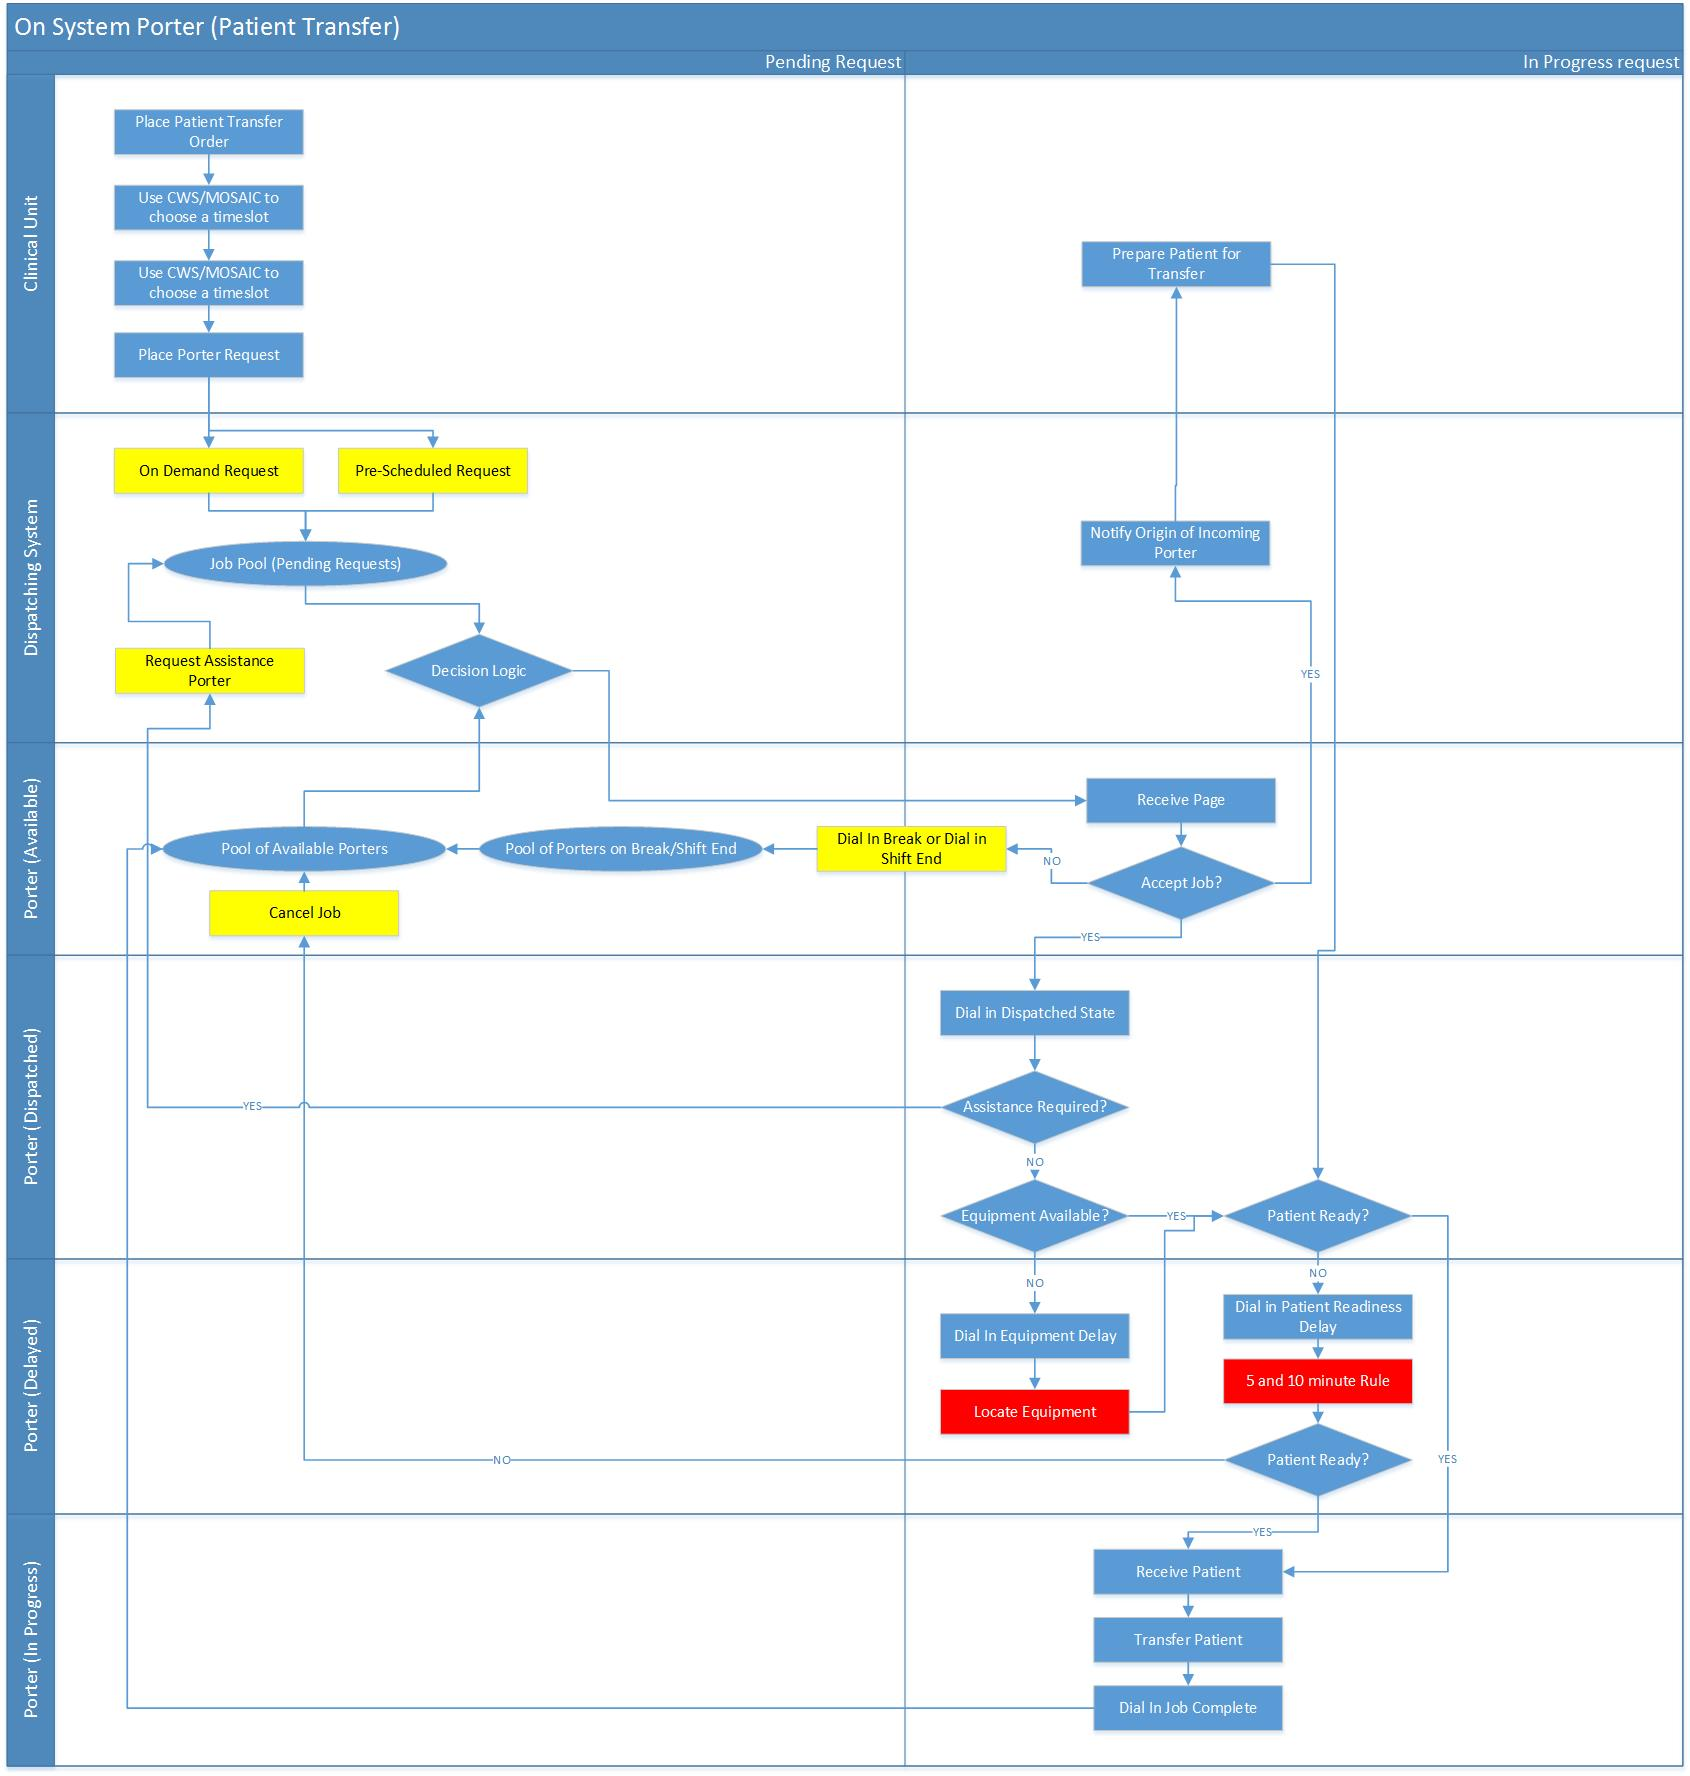
\includegraphics[width=1\textwidth, height=0.8\textheight, keepaspectratio]{../Process_Diagrams/Process_Diagram.jpg}
		\caption{Process Diagram}
	\end{center}
\end{figure}

\section{Dependency Diagram}
\begin{figure}[H]
	\begin{center}
		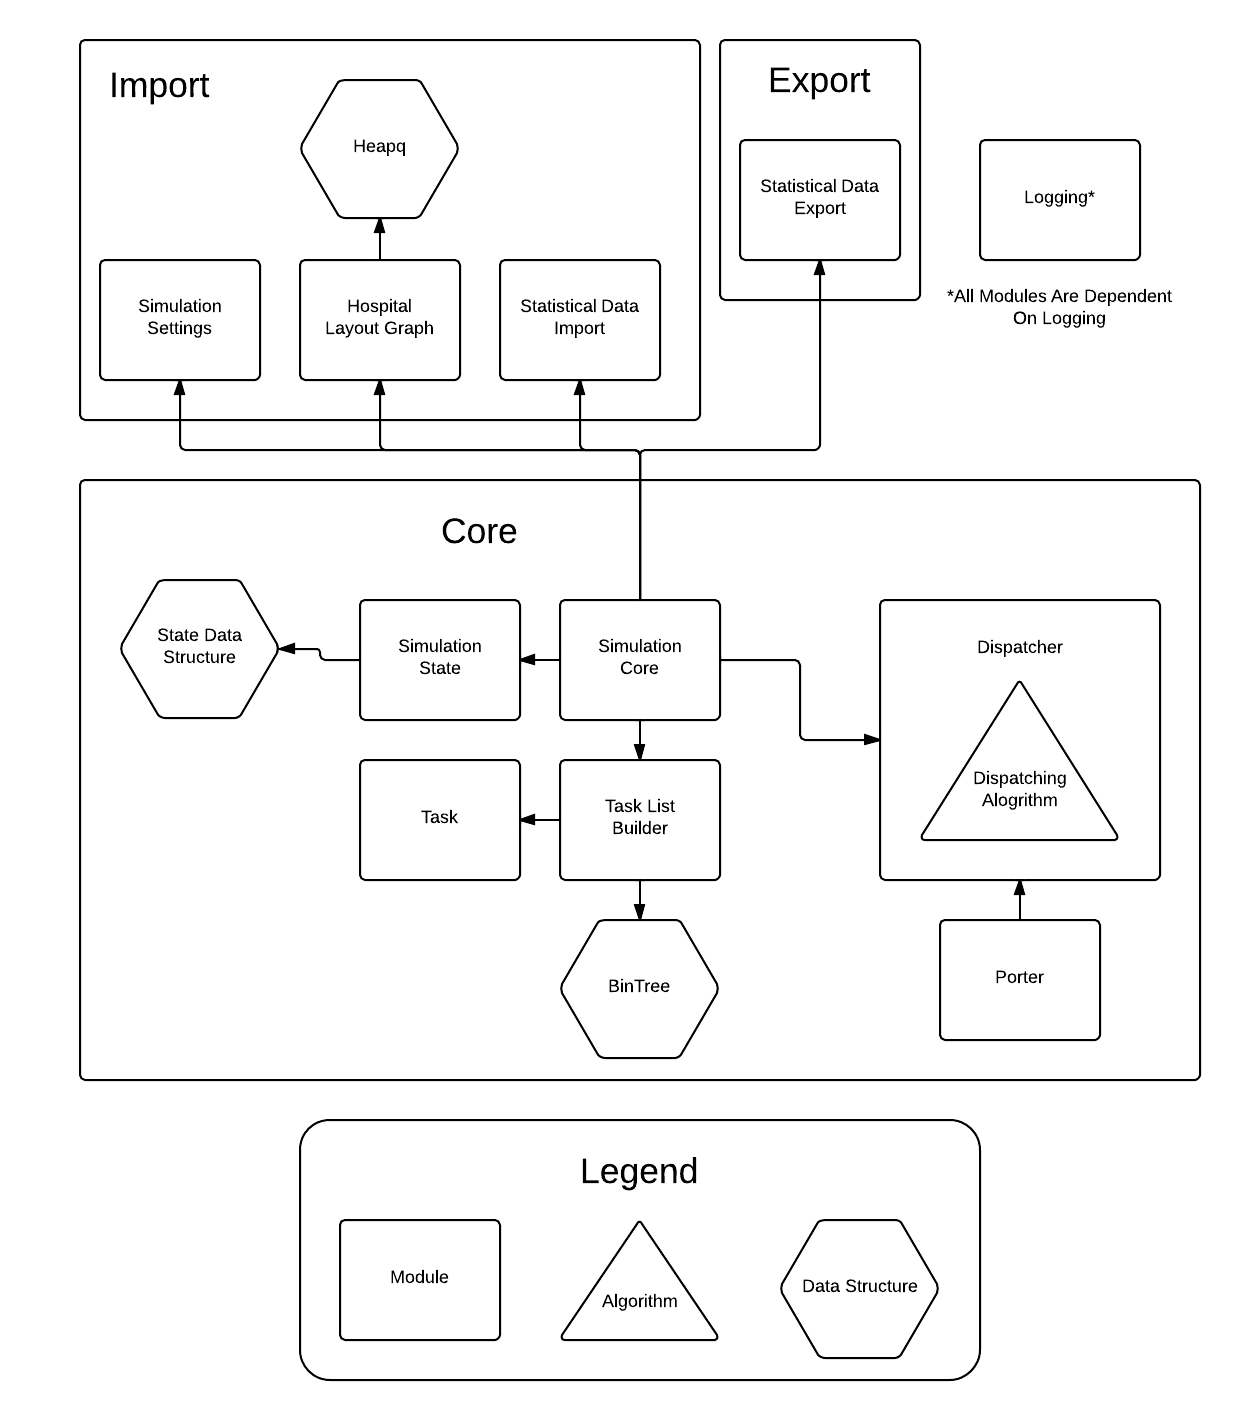
\includegraphics[width=1\textwidth, height=0.8\textheight, keepaspectratio]{../Process_Diagrams/Dependency_Diagram.png}
		\caption{Dependency Diagram}
	\end{center}
\end{figure}

\section{Decomposition Description}
\subsection{Core - Simulation Core}
\begin{enumerate}[]
	\item \textbf{Type:} Module
	\item \textbf{Purpose:} This module calls the required functions to fetch the import data, initializes the simulation and initializes processes.
	\item \textbf{Function:} This module calls the required import modules (Simulation Settings, Hospital Layout Graph, Statistical Data Import), passes their data so that the Simulation State, Event List Builder and Dispatcher can be initialized.
	\item \textbf{Interface:}\\ 
	The interface for the Simulation core is the command line used to called it, defined as follows:
	
	SimCore settings\_filename graph\_filename data\_filename
	
	settings\_filename: the name of the file containing the simulation settings
	
	graph\_filename: the name of the file containing the hospital layout graph
	
	data\_filename: the name of the file containing the statistical data
	
	\item \textbf{Process Steps:} This module first uses the Simulation Settings, Hospital Layout Graph and Statistical data to read in the external data.  This data is used to configure other core modules in the simulation.
	
	Once the external data is imported and the core modules are configured, the Simulation Core will begin the simulation and manage the core modules.
	\item \textbf{Data:} None
	\item \textbf{Error Handling:} Catch all on the simulation loop to report pertinent errors and to prevent unexpected termination. 
	\item \textbf{Requirement Reference:} 11.5.1
	\item \textbf{Critical Revision 0 Component:} True
	\item \textbf{To Be Completed By:} 28/01/2014
	\item \textbf{To Be Tested By:} 30/01/2014
\end{enumerate}
\subsection{Core - Simulation State}
\begin{enumerate}[]
	\item \textbf{Type:} Module
	\item \textbf{Purpose:} This module's purpose is to be an interface between the simulation and its simulation state data structure.
	\item \textbf{Function:} This module will contain functions that will be used by the simulation to perform queries on the simulation state data structure.
	\item \textbf{Interface:}\newline
	initSimulateState():
		\begin{itemize}
			\item Instantiating the simulation state with null values
		\end{itemize}
	getSimulationTime():
		\begin{itemize}
			\item Returns the current simulation time
		\end{itemize}
	getPorterList():
		\begin{itemize}
			\item Returns a list of the porter objects
		\end{itemize}
	getTaskList():
		\begin{itemize}
			\item Returns the task list
		\end{itemize}			
	\item \textbf{Process Steps:} This module handles the simulation state data structure and allows the rest of the modules to interact with it.  If modules need information about the simulation as a whole, they will communicate with the Simulation State module in order to satisfy their needs. 
	\item \textbf{Data:} Simulation state data structure
	\item \textbf{Error Handling:} Catch any null values in the simulation state data structure
	\item \textbf{Requirement Reference:} None
	\item \textbf{Critical Revision 0 Component:} True
	\item \textbf{To Be Completed By:} 28/01/2014
	\item \textbf{To Be Tested By:} 30/01/2014
\end{enumerate}
\subsection{Core - Task}
\begin{enumerate}[]
	\item \textbf{Type:} Module
	\item \textbf{Purpose:} Provide information about a job to the porter.
	\item \textbf{Function:} The task is declared with an origin, destination, required equipment and a priority.  This information is necessary to allowing a porter to complete a job.
	\item \textbf{Interface:} \newline
		getOriginLocation():
			\begin{itemize}
				\item Returns the origin of a job
			\end{itemize}
		getDestinationLocation():
			\begin{itemize}
				\item Returns the destination of a job
			\end{itemize}
		getEquipment():
			\begin{itemize}
				\item Returns the equipment required for a job
			\end{itemize}
		getPriority():
			\begin{itemize}
				\item Returns the priority of a job
			\end{itemize}
		getTime():
			\begin{itemize}
				\item Returns the time that the task will be requested
			\end{itemize}			
		updatePriority():
			\begin{itemize}
				\item A process that will set the job to a higher priority after a specified amount of time has passed.
			\end{itemize}
	\item \textbf{Process Steps:}  Tasks will be initialized once the Simulation Core shares the import modules with the Event List Builder.  An initialized task will be able to provide the Dispatcher all the required information to organize a list of tasks.  Also, once a task is given to a porter, the porter will then be able to start and complete a transport job.
	\item \textbf{Data:} Transport Job Information
	\item \textbf{Error Handling:} Catch any null values returned by the task's properties
	\item \textbf{Requirement Reference:} None
	\item \textbf{Critical Revision 0 Component:} True
	\item \textbf{To Be Completed By:} 28/01/2014
	\item \textbf{To Be Tested By:} 30/01/2014
\end{enumerate}
\subsection{Core - Task List Builder}
\begin{enumerate}[]
	\item \textbf{Type:} Module
	\item \textbf{Purpose:} Produces the list of tasks for the Simulation Core and Dispatcher modules to process
	\item \textbf{Function:} This module populates a series of tasks following either a distribution or statistical data.
	\item \textbf{Interface:} \newline
		addTask(origin, destination, equipment, priority, time):
		\begin{itemize}
			\item Input the origin, destination, equipment and priority of a job.  Also include the time the task will be added to the Dispatcher
		\end{itemize}
		setTaskBuilderStats(data)
		\begin{itemize}
			\item Input the statistical or distribution data as it is required for creating meaningful data
		\end{itemize}
		
	\item \textbf{Process Steps:} The Task List Builder will first receive the data from the Simulation Core.  This data will allow the Task List Builder to create jobs based on user specified parameters.  Secondly, the Task List Builder will generate tasks and append them to the BinTree data structure, to allow for ordering, inserting and retrieval of tasks.  Once a task reaches its "time" it will be added to the Dispatcher where it can be given to an available porter.
	\item \textbf{Data:} Task List BinTree
	\item \textbf{Error Handling:} Catch any null tasks
	\item \textbf{Requirement Reference:} 8.1.4
	\item \textbf{Critical Revision 0 Component:} True
	\item \textbf{To Be Completed By:} 28/01/2014
	\item \textbf{To Be Tested By:} 30/01/2014
\end{enumerate}
\subsection{Core - Porter}
\begin{enumerate}[]
	\item \textbf{Type:} Module
	\item \textbf{Purpose:}  To complete jobs provided by the dispatcher
	\item \textbf{Function:} Completes the transport jobs assigned by the dispatcher.  Unless a job is cancelled the porter will traverse through four states ('pending', 'dispatched', 'inprogress', 'complete')
	\item \textbf{Interface:} \newline
	setStatePending(state):
		\begin{itemize}
			\item Input the pending state
			\item Sets the porter's state to pending and waits to be assigned a job
		\end{itemize}
	setStateDispatched(state):
		\begin{itemize}
			\item Input the dispatched state
			\item Sets the porter's state to dispatched and calculates the time between the porter's location and the job's origin	
		\end{itemize}
	setStateInprogress(state):
		\begin{itemize}
			\item Input the inprogress state
			\item Sets the porter's state to inprogress and calculates the time between the job's origin and destination
		\end{itemize}
	setStateComplete(state):
		\begin{itemize}
			\item Input the complete state
			\item Sets the porter's state to complete, records the completion time and sets the porter back to the pending state
		\end{itemize}
	getAutoLocation():
		\begin{itemize}
			\item Returns the estimated location of a pending porter
			\item Estimates the current location of a porter based on how many minutes they have been in 
			\item Output the estimated location of a pending porter
			\item Estimates the current location of a porter based on how many minutes they have been in the pending state.
		\end{itemize}
	\item \textbf{Process Steps:} The module listens for state changes provided by the dispatcher and updates its' internal components as necessary.
	\item \textbf{Data:} Stores internal data relating to its' current state.
	\item \textbf{Error Handling:} None
	\item \textbf{Requirement Reference:} None
	\item \textbf{Critical Revision 0 Component:} True
	\item \textbf{To Be Completed By:} 28/01/2014
	\item \textbf{To Be Tested By:} 30/01/2014
\end{enumerate}
\subsection{Core - Dispatcher}
\begin{enumerate}[]
	\item \textbf{Type:} Module
	\item \textbf{Purpose:} To organize pending jobs based on a weighted-value and assign them to porters 
	\item \textbf{Function:} This module orders pending jobs based off of a Dispatch Value which is computed using several parameters (Proximity Match Value, Weighted Job Priority and Appointment Factor).  The pending job with the greatest Dispatch Value will be assigned to the closest available porter.  Once the job is assigned to the porter the job will be considered as a dispatched job.
	\item \textbf{Interface:} \newline
	 assignJob(Task):
	 	\begin{itemize}
	 		\item Assigns the job with the greatest Dispatch Value to the closest available porter.
	 	\end{itemize}
	 getProxmityMatchValue(TaskOrigin):
	 	\begin{itemize}
	 		\item Input the origin of a pending job
	 		\item Output a value based on how close an available porter is to a job's origin
	 	\end{itemize}
	 getWeightedJobPriority(TaskOrigin, TaskDestination):
	 	\begin{itemize}
	 		\item Input the origin and destination of a pending job
	 		\item Output a value based on the priority of the pending job
	 	\end{itemize}
	 getAppointmentFactor(Task):
	 	\begin{itemize}
	 		\item Input a pending job
	 		\item Update the value for a job depending on if it was pre-scheduled or on-demand.
	 	\end{itemize}
	 getDispatchValue(Task):
	 	\begin{itemize}
	 		\item Input a pending job
	 		\item Compute the DispatchValue for a job: (ProxmityMatchValue + WeightedJobPriority * AppointmentFactor) 
	 	\end{itemize}
	\item \textbf{Process Steps:}
	All pending jobs are assessed and given a dispatch value (DV) based on the weighting and values of specified dispatch parameters.
	
	These weights and values are determined using either the location of an available porter or the priority of a pending job.
	
	All of the pending jobs are then ordered from greatest dispatch value to the least.  When there is an available porter the pending job with the greatest dispatch value is given to the closest porter.
	\item \textbf{Data:}
		\begin{itemize}
			\item Pending jobs
		\end{itemize}
	\item \textbf{Error Handling:} None
	\item \textbf{Requirement Reference:} None
	\item \textbf{Critical Revision 0 Component:} True
	\item \textbf{To Be Completed By:} 28/01/2014
	\item \textbf{To Be Tested By:} 30/01/2014
\end{enumerate}
\subsection{Import - Simulation Setting}
\begin{enumerate}[]
	\item \textbf{Type:} Module
	\item \textbf{Purpose:} Receives the settings data from the GUI and translates them for use by the simulation core
	\item \textbf{Function:} Receives data in the form of a csv and converts it to a readable format
	\item \textbf{Interface:} \newline
	receiveSettings(Settings):
	 	\begin{itemize}
	 		\item Load and store setting into module
	 	\end{itemize}
	 translateSettings():
	 	\begin{itemize}
	 		\item Outputs translated setting from the current loaded setting in the module
	 	\end{itemize}
	\item \textbf{Process Steps:} the module is called by the GUI from which it receives the settings as a csv file and stores them. Simulation Core calls the module to receive the current setting in the translated format. 
	\item \textbf{Data:} Settings
	\item \textbf{Error Handling:} return NULL on incorrect settings received
	\item \textbf{Requirement Reference:} 8.1.1, 8.1.2
	\item \textbf{Critical Revision 0 Component:} True
	\item \textbf{To Be Completed By:} 28/01/2014
	\item \textbf{To Be Tested By:} 30/01/2014
\end{enumerate}
\subsection{Import - Hospital Layout Graph}
\begin{enumerate}[] 
	\item \textbf{Type:} Module
	\item \textbf{Purpose:} Receives layout data for the hospital from a .csv file and translates it for use by the simulation core.
	\item \textbf{Function:} Interprets the data from the .csv file into a graph representing a HHS hospital transportation layout for porter movement.
	\item \textbf{Interface:} \newline
	receiveLayout(Layout):
	 	\begin{itemize}
	 		\item Load and store layout into module
	 	\end{itemize}
	 translateLayout():
	 	\begin{itemize}
	 		\item Outputs translated layout from the currently loaded .csv file to the module
	 	\end{itemize}
	\item \textbf{Process Steps:} Simulation core calls the module to receive the translated layout.
	\item \textbf{Data:} Layout Graph
	\item \textbf{Error Handling:} Returns NULL on incorrect settings.
	\item \textbf{Requirement Reference:} 8.1.1, 8.1.2
	\item \textbf{Critical Revision 0 Component:} True
	\item \textbf{To Be Completed By:} 28/01/2014
	\item \textbf{To Be Tested By:} 30/01/2014
\end{enumerate}
\subsection{Import - Statistical Data Import}
\begin{enumerate}[]
	\item \textbf{Type:} Module
	\item \textbf{Purpose:} Receives statistical data for the hospital from a .csv file and translates it for use by the simulation core.
	\item \textbf{Function:} Interprets the data from the .csv file into statistical data and places them into variables for use by the Simulation Core.  
	\item \textbf{Interface:} \newline
	receiveStatistics(Statistics):
	 	\begin{itemize}
	 		\item Load and store statistics into module
	 	\end{itemize}
	 translateStatistics():
	 	\begin{itemize}
	 		\item Outputs translated statistics from the currently loaded .csv file to the module
	 	\end{itemize}
	\item \textbf{Process Steps:} Simulation core calls the module to receive the translated statistical data variables.
	\item \textbf{Data:} Statistic data variables
	\item \textbf{Error Handling:} Returns NULL on incorrect settings.
	\item \textbf{Requirement Reference:} 8.1.1, 8.1.2
	\item \textbf{Critical Revision 0 Component:} True
	\item \textbf{To Be Completed By:} 28/01/2014
	\item \textbf{To Be Tested By:} 30/01/2014
\end{enumerate}
\subsection{Export - Statistical Data Export}
\begin{enumerate}[]
	\item \textbf{Type:} Module
	\item \textbf{Purpose:} Format and output the raw data from the simulation.
	\item \textbf{Function:} This module will gather all of the raw data from the simulation and format it  so that it can be exported into a readable excel file.
	\item \textbf{Interface:}
	addExportData(data)
	\begin{itemize}
		\item Input raw data
	\end{itemize}
	publishExportData()
	\begin{itemize}
		\item This function will format the simulation's raw data, create an excel file and populate the file with the formatted data
	\end{itemize}
	\item \textbf{Process Steps:} All data that is to be exported must be added to this module.  Once the simulation's raw data is gathered the module will publish the data.  The publishing will generate an excel file and outline the results from the simulation.
	\item \textbf{Data:} None
	\item \textbf{Error Handling:}  Produce warning message if data is missing during the publishing.
	\item \textbf{Requirement Reference:} 8.1.5
	\item \textbf{Critical Revision 0 Component:} True
	\item \textbf{To Be Completed By:} 28/01/2014
	\item \textbf{To Be Tested By:} 30/01/2014
\end{enumerate}
\subsection{Logging}
\begin{enumerate}[]
	\item \textbf{Type:} Module
	\item \textbf{Purpose:} Provide logging capabilities across all Python modules
	\item \textbf{Function:} This module will contain python's native logging library as well provide any additional logging functionality specific to the simulation.
	\item \textbf{Interface:}
	initializeLogging()
		\begin{itemize}
			\item Initialize python's native logging across the modules
		\end{itemize}
	printLogging(module)
		\begin{itemize}
			\item Print a module's simulation log
		\end{itemize}
	\item \textbf{Process Steps:} A logger will be created for each module providing necessary error tracking.  Not only this but the Logging module will allow for debugging during the course of development.
	\item \textbf{Data:} Module Logs
	\item \textbf{Error Handling:} Catch any null module logs.
	\item \textbf{Requirement Reference:} 13.1
	\item \textbf{Critical Revision 0 Component:} True
	\item \textbf{To Be Completed By:} 28/01/2014
	\item \textbf{To Be Tested By:} 30/01/2014
\end{enumerate}


\subsection{GUI - Basic Settings - General}
\begin{enumerate}[]
	\item \textbf{Type:} User Interface
	\item \textbf{Purpose:} Allows the user to change the basic-general settings of the simulation
	\item \textbf{Function:} 
	\begin{enumerate}[(i)]
		\item \textbf{Simulation Duration:} Number of days the software will simulate events.
		\item \textbf{Porter Wait Times:} Maximum number of minutes a porter waits for a delay (patient, equipment, nurse) before cancelling the job
		\item \textbf{Job Flow:} The rate of event generation during the course of the simulation.
		\item \textbf{Start Day:} Define the first day the simulation generates events from.
	\end{enumerate}
	\item \textbf{Process Steps:} Not Available
	\item \textbf{Data:} Not Available
	\item \textbf{Error Handling:} The interface prevents the user from violating constraints
	\begin{enumerate}[]
		\item \textbf{Simulation Duration:} Value 0 to 7 
		\item \textbf{Porter Wait Times:} Value 0 to 60
		\item \textbf{Job Flow:} Drop down defined by interface {Low, Normal, High}
		\item \textbf{Start Day:} Drop down defined by interface {Monday, Tuesday, Wednesday, Thursday, Friday, Saturday, Sunday}   
	\end{enumerate}
	\item \textbf{Requirement Reference:} 10.1.1, 10.1.2, 10.1.3, 10.1.4
\end{enumerate}

\subsection{GUI - Basic Settings - File Locations}
\begin{enumerate}[]
	\item \textbf{Type:} User Interface
	\item \textbf{Purpose:} Allows the user to choose the directory paths for required import/export files
	\item \textbf{Function:} 
	\begin{enumerate}[(i)]
		\item \textbf{Statistical Data Source:} Determines which source file will be used to provide the simulation with statistical distribution information
		\item \textbf{Schedule Data Source:} Determines which source file will be used to provide scheduling information to be used during simulation
		\item \textbf{Output Location:} Determines the Location to store output data
	\end{enumerate}
	\item \textbf{Process Steps:} Not Available
	\item \textbf{Data:} Not Available
	\item \textbf{Error Handling:} The interface prompts the user with an error message upon entry of erroneous data
	\begin{enumerate}[]
		\item \textbf{Statistical Data Source:} File exists. File extension is ".csv"
		\item \textbf{Schedule Data Source:} File Exists. File extension is ".csv"
		\item \textbf{Output Location:} Directory exists
	\end{enumerate}
	\item \textbf{Requirement Reference:} 10.1.1, 10.1.2, 10.1.3, 10.1.4
\end{enumerate}

\subsection{GUI - Basic Settings - Buttons/Output Console}
\begin{enumerate}[]
	\item \textbf{Type:} User Interface
	\item \textbf{Purpose:} Allows the user to activate simulation or reset all data
	\item \textbf{Function:} 
	\begin{enumerate}[(i)]
		\item \textbf{Simulate Button:} Runs all the integrity checks and initializes the simulation run
		\item \textbf{Reset All Button:} Resets all data to initial values
		\item \textbf{Output Console:} Prints any logging statements
	\end{enumerate}
	\item \textbf{Process Steps:} Not Available
	\item \textbf{Data:} Not Available
	\item \textbf{Error Handling:} Interface prevents user from entering erroneous data 
	\begin{enumerate}[]
		\item \textbf{Output Console:} Console is read only
	\end{enumerate}
	\item \textbf{Requirement Reference:} 10.1.1, 10.1.2, 10.1.3, 10.1.4
\end{enumerate}

\subsection{GUI - Advanced Settings - Dispatcher/Random Seed}
\begin{enumerate}[]
	\item \textbf{Type:} User Interface
	\item \textbf{Purpose:} Allows the user to tool around with dispatcher values
	\item \textbf{Function:} 
	\begin{enumerate}[(i)]
		\item \textbf{Appointment Factor:} 
		\item \textbf{Automatic Job Priority Values:} 
		\item \textbf{Weighted Job List:} 
		\item \textbf{Random Seed:} allows the user to enter a specific random seed instead of true random
	\end{enumerate}
	\item \textbf{Process Steps:} Not Available
	\item \textbf{Data:} Not Available
	\item \textbf{Error Handling:} Interface prevents user from entering erroneous data 
	\begin{enumerate}[]
		\item \textbf{Appointment Factor:} Value 0.0 to 3.0
		\item \textbf{Automatic Job Priority Values:} Values 0.0 to 99.99
		\item \textbf{Weighted Job List:} Values 0.0 to 99.99
		\item \textbf{Random Seed:} Value 0 to 999999999
	\end{enumerate}
	\item \textbf{Requirement Reference:} 10.1.1, 10.1.2, 10.1.3, 10.1.4
\end{enumerate}

\subsection{Schedule Verifier}
\begin{enumerate}[]
	\item \textbf{Type:} Module
	\item \textbf{Purpose:} Confirms the integrity of the schedule
	\item \textbf{Function:} 
	\begin{enumerate}[(i)]
		\item \textbf{scheduleChecker(file):} checks integrity of the schedule as a whole
		\item \textbf{verifyShiftID(element):} checks integrity of each shift id  
		\item \textbf{verifyStartTime(element):} checks integrity of each start time 
		\item \textbf{verifyEndTime(element):} checks integrity of each end time 
		\item \textbf{verifyPorterID(element):} checks integrity of each porter id 
		\item \textbf{verifyDays(element):} checks integrity of each day entry
	\end{enumerate}
	\item \textbf{Process Steps:} scheduleChecker opens the schedule file and verifies each element of the file with a subroutine
	\item \textbf{Data:} schedule data file
	\item \textbf{Error Handling:} Module gathers and returns all the errors
	\begin{enumerate}[]
		\item \textbf{scheduleChecker(file):} returns the returns from all the subroutines (returns the cell and place of error)
		\item \textbf{verifyShiftID(element):} string of character [A-Za-z0-9] 
		\item \textbf{verifyStartTime(element):} is date
		\item \textbf{verifyEndTime(element):} is date
		\item \textbf{verifyPorterID(element):} string of character [A-Za-z0-9] 
		\item \textbf{verifyDays(element):} value 0 - 6
	\end{enumerate}
	\item \textbf{Requirement Reference:} ??
\end{enumerate}

\subsection{Schedule Parser}
\begin{enumerate}[]
	\item \textbf{Type:} Module
	\item \textbf{Purpose:} Converts the schedule to a more convenient format
	\item \textbf{Function:} 
	\begin{enumerate}[(i)]
		\item \textbf{scheduleParser(file):} checks integrity of the schedule as a whole
	\end{enumerate}
	\item \textbf{Process Steps:} scheduleParser opens the schedule file and converts it to a python dictionary format
	\item \textbf{Data:} schedule data file
	\item \textbf{Error Handling:} No error if Schedule Verifier has been executed
	\item \textbf{Requirement Reference:} ??
\end{enumerate}

\section{Anticipated Changes}
None

\section{Appendicies}
\subsection{Figure Appendix}
\begin{enumerate}[(a)]
	\item Figure 4.1: Process Diagram.jpg - the process flow diagram details the process modeled by the simulation.
	\item Figure 5.1: Dependency Diagram.png - layout of the module, algorithm and data structure dependencies.
	\item Figure 6.1: Basic GUI.png - prototype design of the GUI associated for use with the simulation.
\end{enumerate}
\subsection{Algorithm Appendix}
\begin{enumerate}[(a)]
	\item Dispatching Algorithm - main dispatcher algorithm used to assign jobs to porters based on a number of factors. Functionality outlined by section 6.6 of this document.
	\item Dijkstra's Algorithm - will be used to compute the shortest path between two hospital location.
\end{enumerate}

%%% End document
\end{document}